
Para poder empezar la descripción primero hay que presentar una explicación del vocabulario básico. Lo cierto es que acerca de DDD y arquitecturas de software hay ingente documentación. Realizar un exposición de toda la teoría sería extenso. Como referencia fundamentar para iniciarse en el tema tomamos como referencia la devopedia\cite{devopediaDDD}. Intentar resumirlo mejor carece de valor. Este trabajo lo que intenta no es ser un manual teórico más de DDD, si no una aplicación práctica de dichos conceptos para entender en un caso real el alcance de dicha teoría. Las referencias básicas que se van a tomar son:

\begin{itemize}
    \item Domain-Driven Design: Tackling Complexity in the Heart of Software. De Eric Evans\cite{EricEvans2003DDTC}
    \item Implementing Domain-Driven Design. De Vaughn Vernon\cite{VaughnVernon2013IDD}
    \item Get Your Hands Dirty on Clean Architecture de Tom Hombergs \cite{TomHombergs2019GYHD}
\end{itemize}

Toda teoría del DDD va enfocada a desarrollar un lenguaje común a todos los interesados que intervienen en un problema y su solución: clientes, vendedores, técnicos, financieros, etc. para desarrollar ese lenguaje se divide el problema en contextos delimintados. En un ejemplo rápido afiliado en un club deportivo significa facturas, números de identificación fiscal para los financieros y para la gente de operaciones significa reserva de pistas y cancelaciones. y para los de ventas significan descuentos, promociones. Ect. El tener un lenguaje común donde todos puedan expresarse y hablar de la misma solución es el reto de este proceso. Es lo que se define como \textbf{Ubiquitous Language} o \textbf{UL}

Intentar expresar en un mismo contexto todos esos significados termina en lo que se conoce como ¨Big Ball of Mud¨ o Gran bola de barro. Los componentes de este UL se pueden apreciar en la figura  \ref{fig:DomainDrivenDesignReference}, se puede apreciar también la relación entre ellos

\begin{figure}[H]
    \centering
    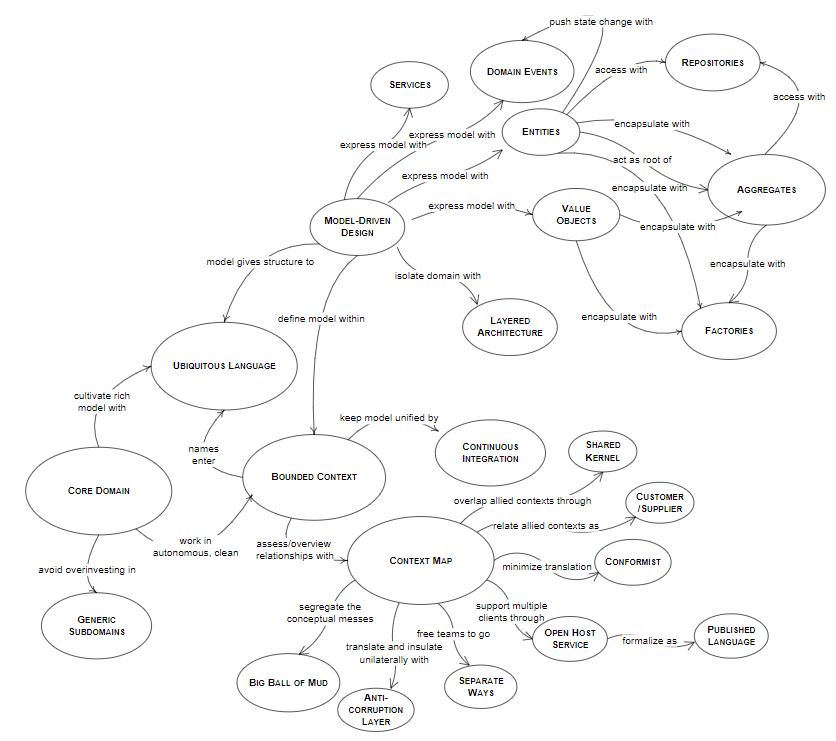
\includegraphics[height=0.5\textheight]{./part/Proyecto_ejecutivo/memoria_descriptiva/infoPreviaAntecedentes/img/DomainDrivenDesignReference}
    \caption{DomainDrivenDesignReference\cite{EricEvans2003DDTC}}\label{fig:DomainDrivenDesignReference}
\end{figure}

De todo este diagrama los conceptos en los que nos vamos a centrar

\begin{itemize}
    \item Entity: Un Objeto que tiene atributos pero principalmente definido por un identificador
    \item Value Object: Un Objeto que tiene atributos pero no identificador
    \item Domain Event: Un Objeto que define una suceso inducido por la interacción entre los componentes del dominio.
    \item Aggregate: Es un cluster de objetos tratado como una unidad. Las referencias o acciones externas sobre sus elementos siempre se hacen a través de un único elemento de este cluster conocido como Aggregate root. Tiene reglas definidas de consistencia dentro de su delimitación. External references are restricted to only one member, called the Aggregate Root.
    \item Repository: Es un mecanismo de interaccion para encapsular el acceso a tecnologías, normalmente de almacenamiento para interactuar con ellas, cuya implementación no concierne al dominio.
    \item Service: Es una funcionalidad de interacción con el dominio que garantiza la interacción con el mismo de una forma consistente
\end{itemize}

Esta definición de dominio se implementa normalmente con un paradigma de diseño conocido como arquitectura de capa. Lo que se busca es aislar esos contextos que definen nuestro dominio de implementaciones concretas ya sea para acceder al mismo o a las que accede el dominio. Por ejemplo, aislarlo de que se ejecute un servicio mediante una consola de comandos o desde una llamada http y que se guarde en una base de datos la información o se guarde en un archivo.

El tipico diagráma cuando se habla de arquitectura hexagonal es tal y como se muestra en la figura\ref{fig:hexagonalDiagram} Si bien consideramos que no tiene mucho sentido y de cara a la parte didáctica confunde, ya que el hexágono es una simple licencia estética. en el caso de existir más puertos de salida y entrada que los representados el hexágono pierde todo el sentido y cuando se enfrenta por primera vez este diagrama se tiende a intentar descifrar el sentído del hexagono.

\begin{figure}[H]
    \centering
    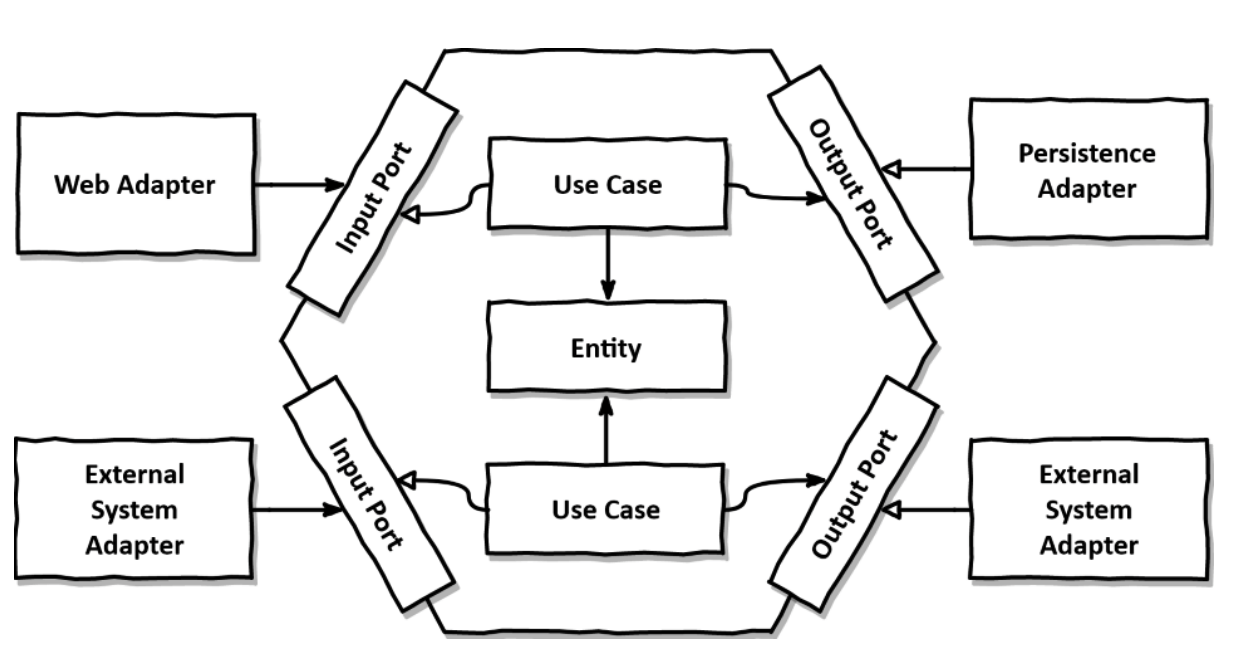
\includegraphics[height=0.3\textheight]{./part/Ejecucion/Seguimiento/CreateTaskUseCase/img/HexagonalDiagram}
    \caption{Hexagonal architecture diagram\cite{TomHombergs2019GYHD}}\label{fig:hexagonalDiagram}
\end{figure}

Vemos en este diagrama que el dominio, representado por la Entity no accede a elementos exteriores. La aplicación respresentada por los UseCase utiliza el dominio y depende de él. pero se aisla del exterior, la infraestructura obligando a utilizar interfaces a los elementos que acceden a el y obligando a implementar las interfaces definidas por la aplicación para la infraestructura que sirve para acceder al exterior de la aplicación.

En el diagrama \ref{fig:layers} podemos ver simplificado que el objetivo es que la dependencia de las capas, expresada por las flechas, sea siempre de fuera hacia adentro. Queremos preservar del cambio el interior y exponer al cambio el exterior. Separar lo propenso al cambio de lo que no. El UL de los detalles de implementación que tienen su propio lenguaje.

\begin{figure}[H]
    \centering
    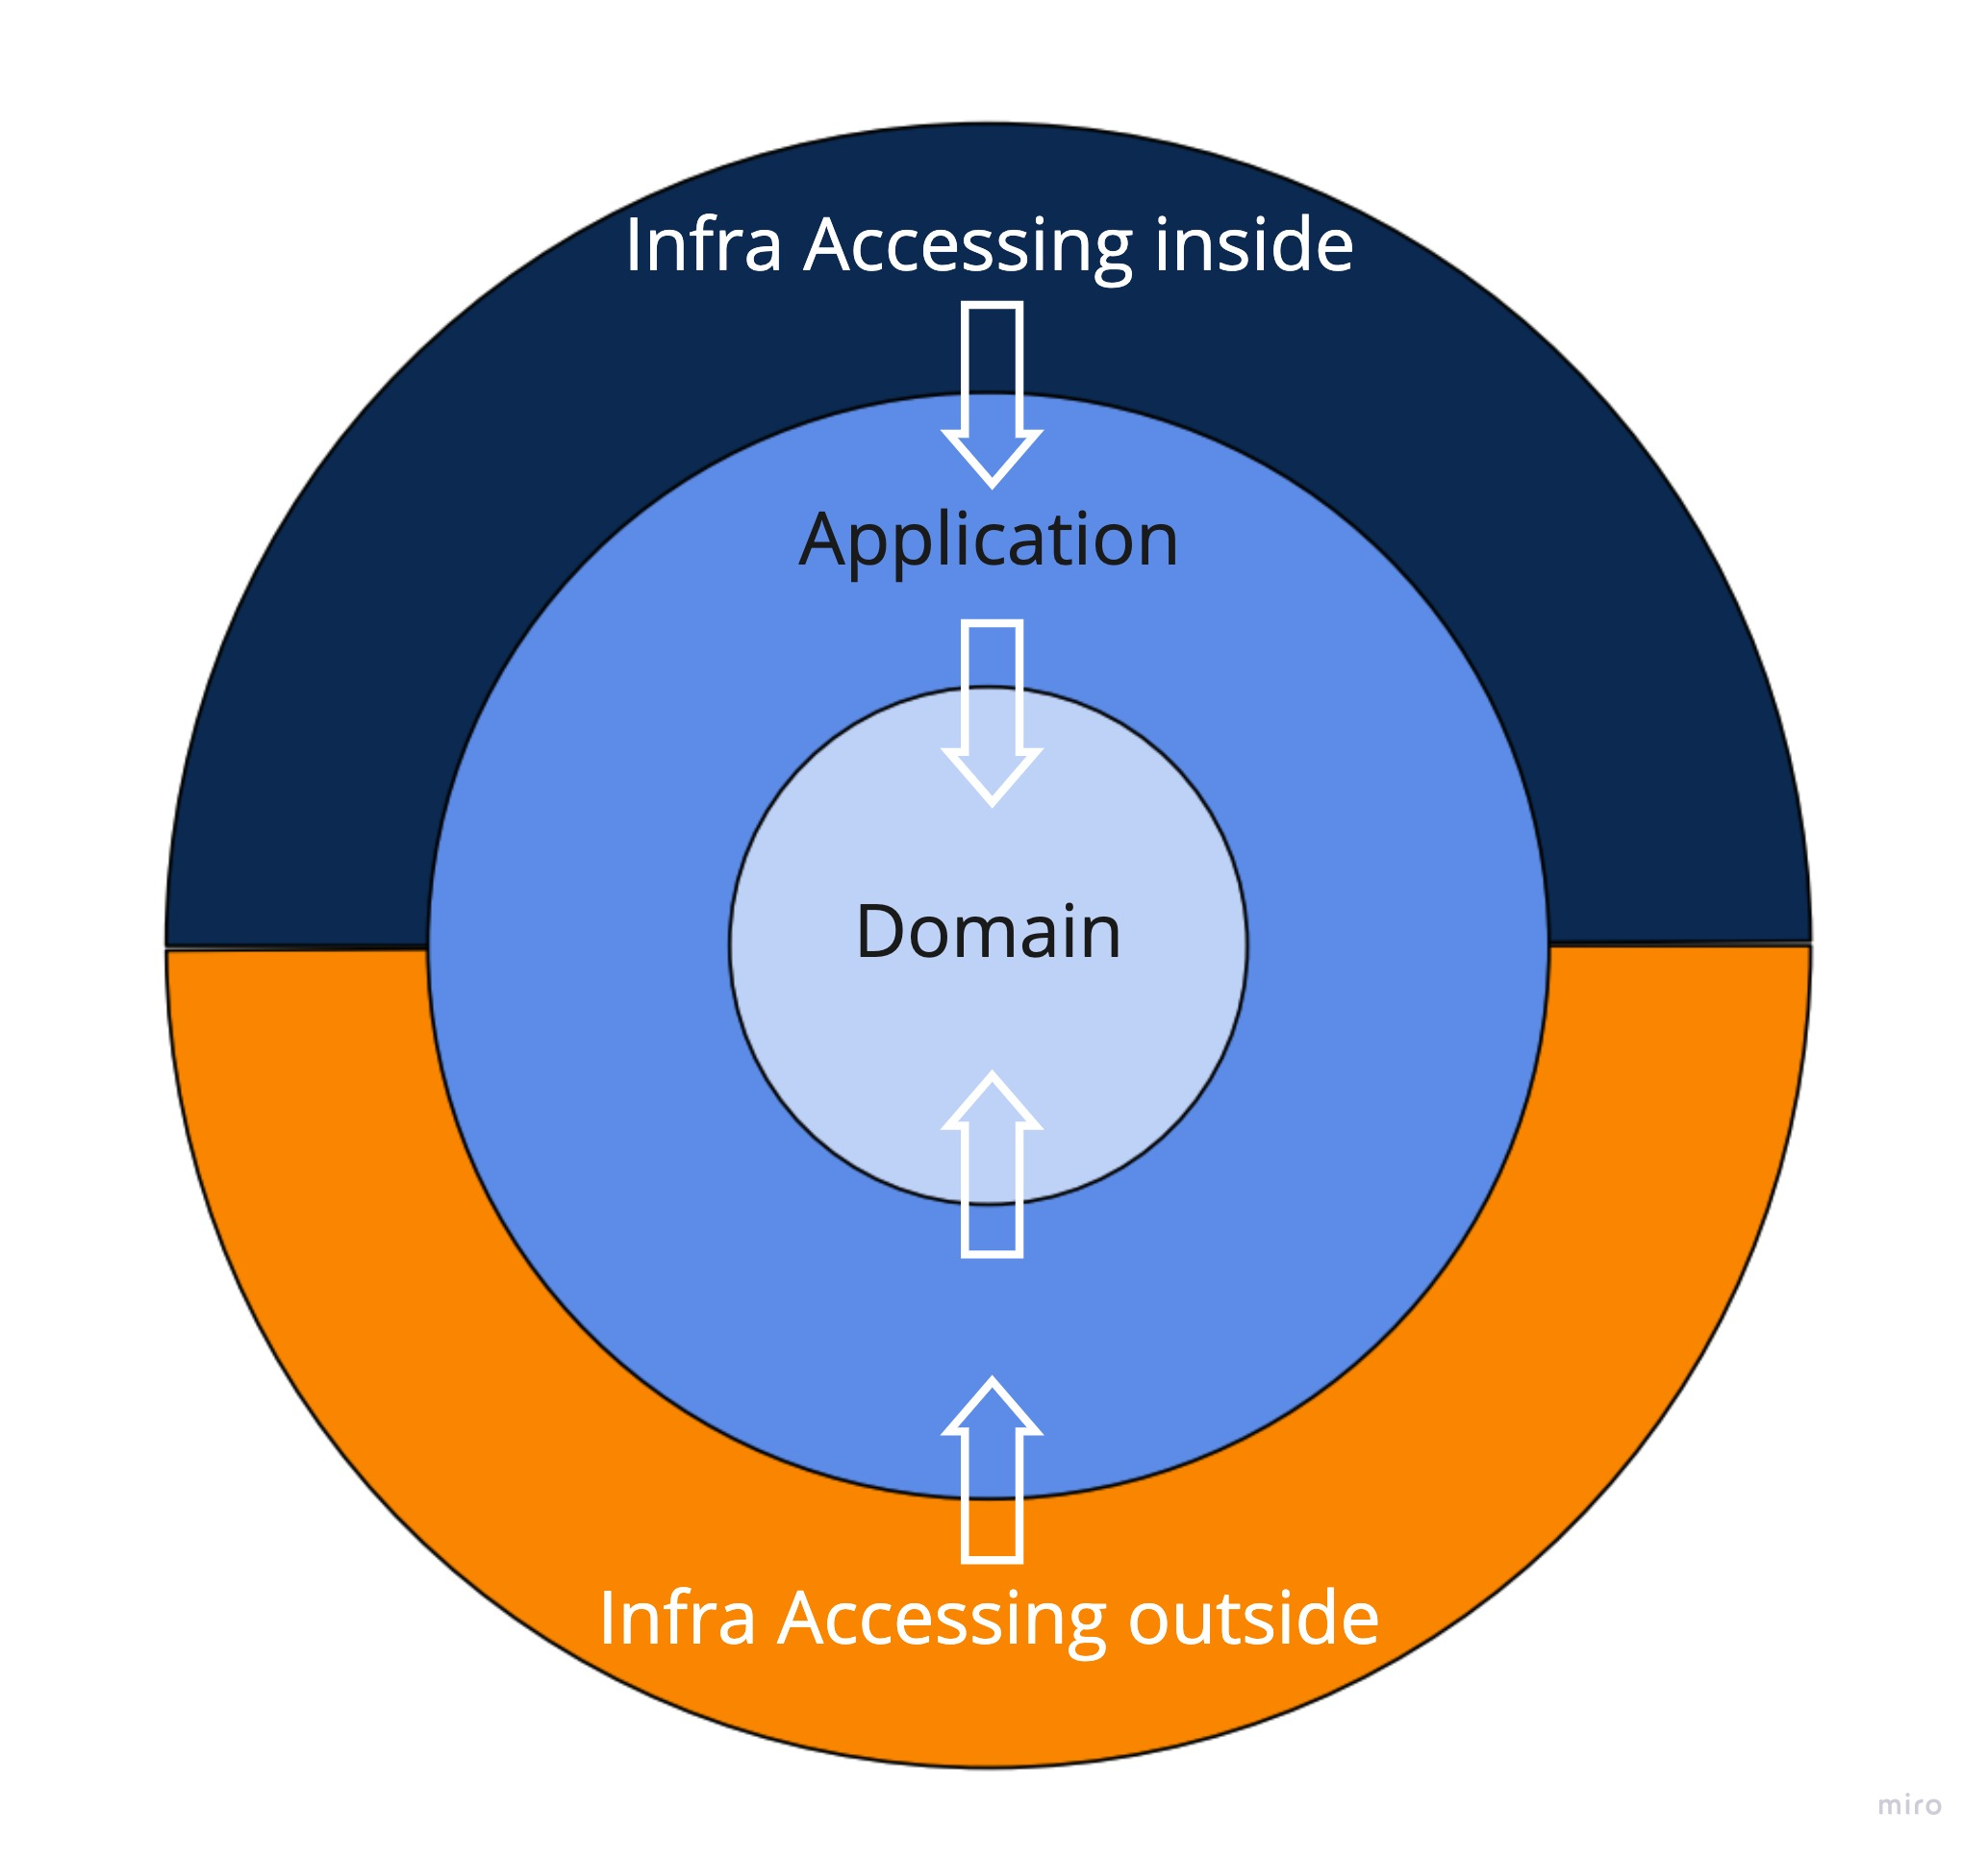
\includegraphics[height=0.3\textheight]{./part/Proyecto_ejecutivo/memoria_descriptiva/infoPreviaAntecedentes/img/PFM - Layer}
    \caption{layered architecture}\label{fig:layers}
\end{figure}

Junto con el concepto de arquitectura hexagonal y el DDD vamos a aplicar el paradigma de diseño conocido como CQRS

CQRS significa Command Query Responsibility Segregation (Segregación de responsabilidades de comandos y consultas, en español). Es una técnica de diseño de arquitectura de software que separa la lógica de escritura (comandos) de la lógica de lectura (consultas) en sistemas de información.

La idea es que las operaciones de escritura (comandos) y las operaciones de lectura (consultas) se manejen por separado, ya que tienen necesidades y características distintas. Mientras que las operaciones de escritura son responsables de modificar el estado de la aplicación, las operaciones de lectura son responsables de devolver información sobre ese estado.

Al separar estas dos responsabilidades, se pueden optimizar las operaciones de lectura para que sean más rápidas y escalables. Además, se puede diseñar una arquitectura de software más flexible, permitiendo una mayor adaptabilidad y evolución del sistema a medida que cambian los requisitos de la aplicación.

Tenemos entonces que vamos a diseñar una arquitectura hexagonal con un enfoque DDD en el dominio y un enfoque CQRS en los casos de uso. Es decir se diseñará un dominio rico y con un UL y se accederá a su funcionalidad a través de casos de uso que sigan el criterio de ser comandos o queries.

Una vez definidas las tres capas y resumido el concepto. Un punto importante a comentar es el concepto de la estrategia de mapping que hay entre capas. Cada capa requiere sus objetos de trabajo para estar desacoplada de las demás. Pero como en todo aspecto está sometido a discusión acerca de seguir la teoría a rajatabla y el pragmatismo de no verse envuelto en redundancias y sobredimensionar las soluciones.

En un extracto del libro Get Your Hands Dirty on Clean Architecture\cite{TomHombergs2019GYHD} podemos leer:
"\textit{ The argument might have gone something like this:}

\begin{itemize}
    \item \textit{Pro-Mapping Developer:}
    \subitem  \textit{ If we don’t map between layers, we have to use the same model in both layers which means that the layers will be tightly coupled!}
    \item \textit{Contra-Mapping Developer:}
    \subitem \textit{ But if we do map between layers, we produce a lot of boilerplate code which is overkill for many use cases, since they’re only doing CRUD and have the same model across layers anyways!}
\end{itemize}
\textit{As is often the case in discussions like this, there’s truth to both sides of the argument. Let’s discuss some mapping strategies with their pros and cons and see if we can help those developers make a decision.}"

Hay tantas estrategias como atajos dentro de este paradigma queramos asumir. Los tipos de mapping que se documentan en este libro:

\begin{itemize}
    \item The NoMapping Strategy \ref{fig:nomapping}
    \item The Two-Way MappingStrategy \ref{fig:twowaymapping}
    \item The Full MappingStrategy \ref{fig:fullmapping}
    \item The One-Way MappingStrategy \ref{fig:onWaymapping}
\end{itemize}

En todos estos casos vemos simplificado el dominio a una única entidad Account y vemos como separa dicho dominio del acceso al proceso que envía dinero a una cuenta y de dónde se guarda la información del envío de ese dinero.

\begin{figure}[H]
    \centering
    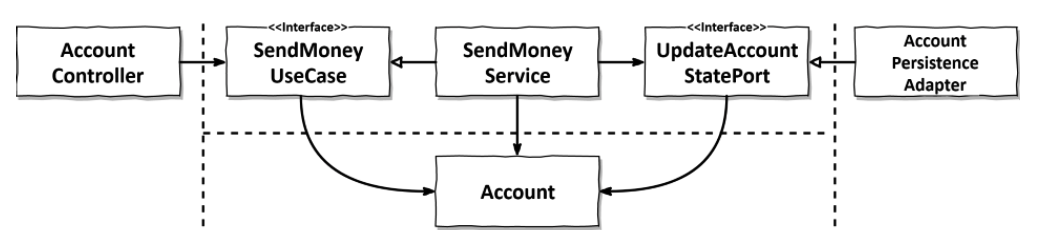
\includegraphics[height=0.1\textheight]{./part/Ejecucion/Seguimiento/CreateTaskUseCase/img/nomapping}
    \caption{No mapping strategy \cite{TomHombergs2019GYHD}}\label{fig:nomapping}
\end{figure}

\begin{figure}[H]
    \centering
    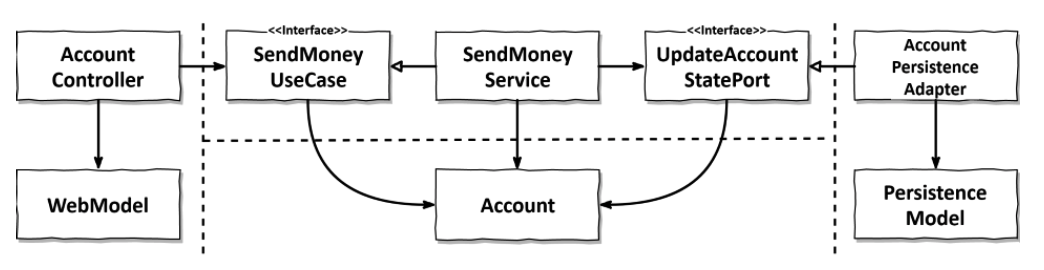
\includegraphics[height=0.1\textheight]{./part/Ejecucion/Seguimiento/CreateTaskUseCase/img/twowaymapping}
    \caption{two way mapping strategy \cite{TomHombergs2019GYHD}}\label{fig:twowaymapping}
\end{figure}

\begin{figure}[H]
    \centering
    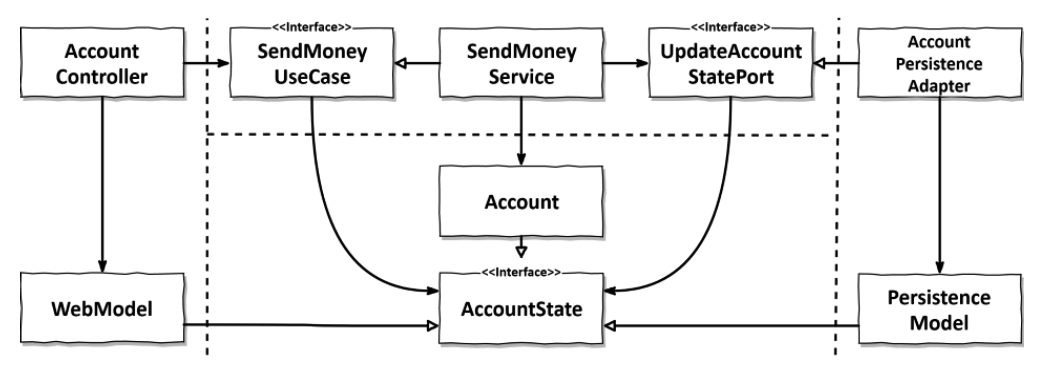
\includegraphics[height=0.1\textheight]{./part/Ejecucion/Seguimiento/CreateTaskUseCase/img/onWaymapping}
    \caption{One way mapping strategy \cite{TomHombergs2019GYHD}}\label{fig:onWaymapping}
\end{figure}

\begin{figure}[H]
    \centering
    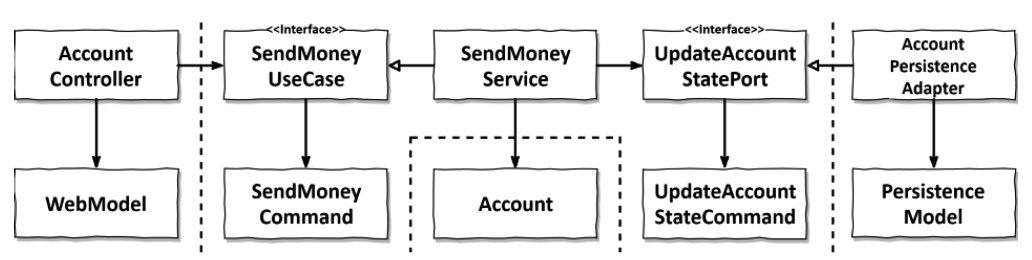
\includegraphics[height=0.1\textheight]{./part/Ejecucion/Seguimiento/CreateTaskUseCase/img/fullmapping}
    \caption{Full mapping strategy \cite{TomHombergs2019GYHD}}\label{fig:fullmapping}
\end{figure}

Todo programa creado en este proyecto: gestor de tareas, cliente y controlador va a estar dividido por tanto en dichas capas y seguir los paradigmas de diseño aquí definidos. En cuanto a la estrategia de mapping tomaremos una decisión cuando nos enfrentemos al problema.